\chapter{Introdução}
A sociedade está lidando com uma quantidade de dados cada vez maior. Hoje, por menor que seja o dado, ele se torna importante pelas informações que podem ser extraídas a partir dele. Se pararmos para pensar, estamos envolvidos por uma quantidade de dados enorme. Como a necessidade de extrair informação é comum em um mundo globalizado e informatizado,  os cientistas e engenheiros se veem obrigados a desenvolvem novas maneiras de medir eventos. Sensores, câmeras de trânsito, dados da web, genes, dados geográficos, dados de compras, dados de pesquisas, e muitas outras informações se tornaram o diferencial nesse mundo competitivo e dinâmico, e precisam de tratamento e atenção~\cite{initBigData}. Conforme Borkar et al ~\cite{WNextBigData} exemplificou, hoje empresas estão monitorando compras de clientes, pesquisas de produtos, sites de relacionamento e diversas outras fontes para aumentar a eficácia do seu marketing e dos serviços ofertados aos clientes, que cada vez mais precisam ser diferenciados e inovadores; governos e empresas estão rastreando conteúdos de blogs e tweets para realizar análises de sentimentos e organizações públicas de saúde estão monitorando artigos de notícias, tweets, e tendências de pesquisas na web para acompanhar o progresso de epidemias~\cite{WNextBigData}.Essa enorme quantidade de dados já gerou, e ainda gera, muitos desafios para cientistas e estudiosos. Não é de hoje que o mundo da TI vem enfrentando grandes problemas com essa grande e heterogênea massa de dados.

No decorrer da evolução dos computadores e com a informatização do mundo, podemos perceber que, ao longo do tempo, a definição de “grande” foi mudando significativamente. Na figura \ref{fig:hd} podemos ter uma idéia dessa evolução.Poucos anos atrás falar em terabytes era coisa de outro mundo, e atualmente a grande maioria das pessoas já possuem dispositivos de armazenamento com capacidade superior a um terabyte. Hoje, para as grandes empresas, já é normal gravar dados na ordem de petabytes (Tabela \ref{tab:bytes}).

	\begin{figure}[!htbp]
		\begin{center}
			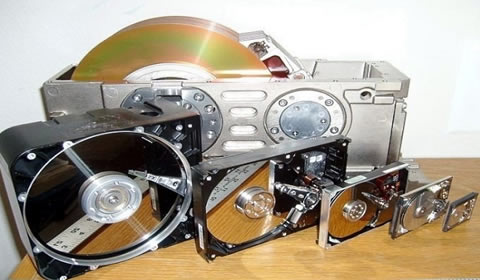
\includegraphics[width=0.8\textwidth]{historiaDiscoRigido}
		\end{center}
		\caption{Evolução do HD ~\cite{hd}}
		\label{fig:hd}
	\end{figure}

Como exemplo podemos citar a administração pública, que possui um grande volume de documentos que precisam ser armazenados com qualidade e cuidado, pois fazem parte dos chamados arquivos permanentes. Esses arquivos ocupam cada vez mais espaço e, devido a sua característica, precisam ser mantidos em locais próprios e com características bem definidas, já que precisam durar por um longo período de tempo. Inúmeras vezes os órgãos precisam consultar esses arquivos e essas consultas, além de contribuírem para a deteriorização dos documentos, são muitas vezes lentas e dificeis de se realizar~\cite{arqConarq}.

A dificuldade de manter esses papéis fez com que o governo federal incentivasse a organização pública a iniciar um processo de digitalização dos documentos para que uma cópia digital desse arquivos fosse mantida pelos órgãos. A digitalização dos arquivos não só possibilita a preservação dos documentos, pois restringe o manuseio dos originais, quanto também facilita o acesso, já que passa a permitir acessos tanto locais quanto remotos e também acessos simultâneos. O processo de digitalização é complexo, demorado e, além de um controle de work flow bem definido, necessita de grandes investimentos de software e hardware para que o resultado tenha uma boa qualidade~\cite{arqConarq}.

Como podemos ver, as finalidades da extrasão desses dados são diversas e podemos retirar informações preciosas dos dados que nos cercam, mas isso nem sempre é trivial e muitas vezes envolve muita tecnologia e estudo. Hoje, além de lidarmos com uma grande quantidade de dados, as vezes nos deparamos com dados que possuem grande variedade e fluxo. Essa massa de dados com características singulares é chamada de big data.

Podemos dividir as tecnologias que sustentam big data em duas: as envolvidas com análise dos dados, como Hadoop e MapReduce e tecnologias de armazenamento e processamento dos dados~\cite{ibmvcsabeoqebigdata}. Na parte de armazenamento podemos citar os bancos de dados NoSql (Not only SQL), que surgiram a partir da necessidade de inovar no que diz respeito ao armazenamento de big data e distribuição de dados.

Dado esse cenário, os SGBDs relacionais não foram capazes de resolver todos os problemas e com o surgimento desse novo paradigma de modelagem, os sitemas de banco de dados NoSql estão sendo cada vez mais utilizados. Como essa tecnologia não-relacional é relativamente recente, existem poucos estudos comparativos que mostre em qual cenário se aplica o uso de uma tecnologia NoSqll e até que ponto ela é melhor que um banco de dados convencional.

Esse trabalho surgiu de uma dúvida arquitetural para a implementação de um sistema que armazenasse todos os dados de servidores públicos federais. Como dito anteriormente, o governo tem orientado os órgãos a digitalizarem os seus arquivos e essa orientação fez com que os órgão se juntassem, devido ao elevado custo para implementação, para darem início a essa conversão dos arquivos físicos em digitais.

O conceito de documentos descentralizados em pastas funcionais será substituído por repositórios de dados e informações de origem primária, auditáveis e não replicados. Com isso teve origem o Projeto de Assentamento Funcional Digital – AFD, que objetiva a criação de um Dossiê, em mídia digital, que será tratado como Fonte Primária de Informação de dados cadastrais do Servidor Público Civil Federal e que substituirá a tradicional Pasta Funcional ou Assentamento Funcional. No site do SIGEPE (Sistema de Gestão de Pessoas) ~\cite{siteSIGEPE} alguns pontos de melhoria com a criação do AFD como: “A criação do Assentamento Funcional Digital (AFD) possibilitará a diminuição drástica do volume de papeis armazenados e tramitados. O AFD constituirá de um banco referencial, de dados e imagens das pastas funcionais, com indexadores para localização dos documentos de maneira online" ~\cite{apresentAFD}.

Para que a base de dados possa cumprir com o seu propósito, ela precisa ter um alto nível de performace, e também, grande escalabilidade. Sendo assim, esse trabalho tem como objetivo analisar a diferença de performace entre bancos de dados NoSql e um banco de Dados Relacional para a gerência dos dados dos servidores públicos.

Para cumprir esse objetivo, desenvolveremos um webservice que possua métodos simples de inserção, consulta, exclusão e atualização de dados. A camada de persistência será implementada em diferentes SGBDs. Testaremos o desempenho da nossa aplicação usando um banco de dados relacional e compararemos o resultado com o de quatro bancos de dados NoSQL com diferentes tipos de modelagem.
